\section{Problem Formulation}
\label{sec:formulation}

This section formulates vehicle scheduling at a general conflict area and then introduces platoon-based scheduling. The presentation follows the physical order of the problem: vehicles first arrive from mutually conflicting approaches, a passing sequence determines how they use the shared conflict area, and grouping consecutive vehicles into platoons restricts the admissible passing sequences.

\subsection{General conflict area and vehicles}

Let \(\approaches=\{1,\ldots,L\}\) denote the set of mutually conflicting approaches. Approach \(l\in\approaches\) contains \(n_l\) vehicles indexed in FIFO order by \((l,i)\), where \(i=1,\ldots,n_l\). The complete vehicle set is
\begin{equation}
\vehicles=\{(l,i):l\in\approaches,\ i=1,\ldots,n_l\},
\end{equation}
and the total number of vehicles is
\begin{equation}
N=\sum_{l\in\approaches}n_l.
\label{eq:total-vehicles}
\end{equation}

Let \(r_{l,i}\) denote the earliest time at which vehicle \((l,i)\) can enter the conflict area if it is not delayed by a preceding vehicle or a vehicle from another approach. These earliest passing times are also referred to as release times. They are assumed to respect the physical FIFO order on each approach:
\begin{equation}
r_{l,i}\le r_{l,i+1},
\qquad l\in\approaches,\quad i=1,\ldots,n_l-1.
\label{eq:fifo-release-times}
\end{equation}
This assumption allows equal release times, for example when several vehicles are queued before the scheduling horizon begins.

\begin{figure}[t]
  \centering
  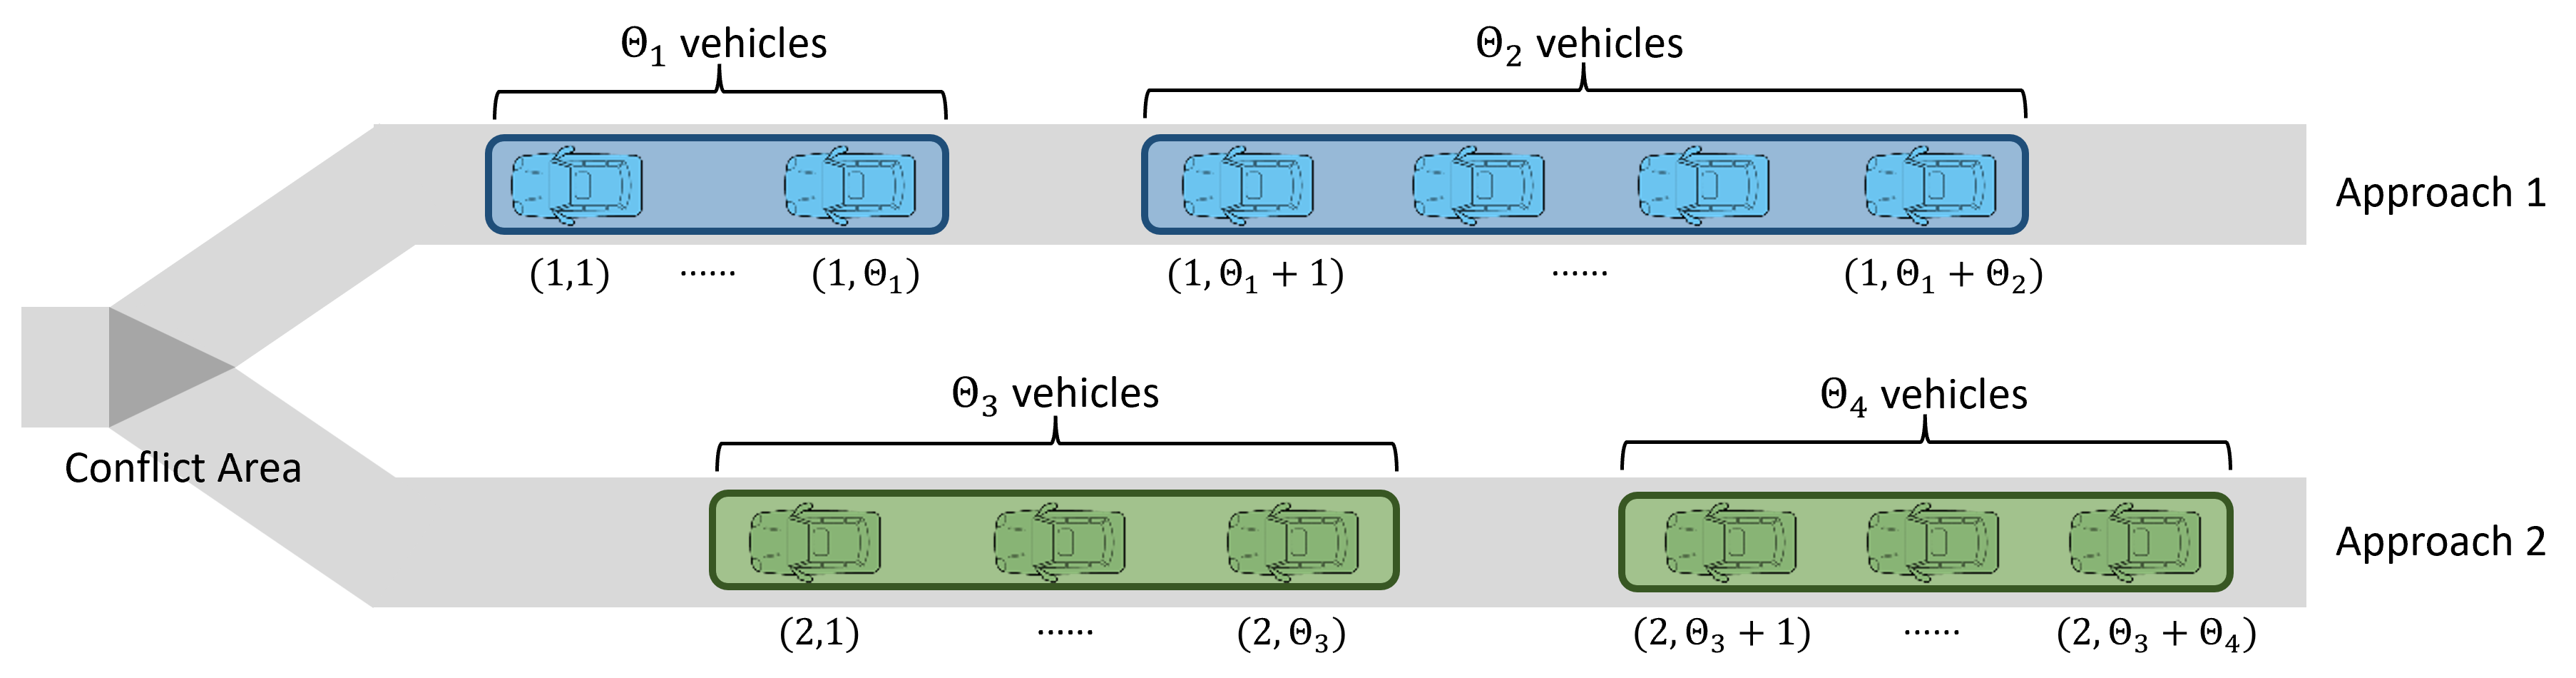
\includegraphics[width=0.95\linewidth]{figures/Picture2.png}
  \caption{Illustration of vehicles approaching a shared conflict area. Vehicles are indexed by approach and FIFO position, and each approach queue may be divided into contiguous platoons.}
  \label{fig:general-conflict-area-platoons}
\end{figure}

Figure~\ref{fig:general-conflict-area-platoons} illustrates the indexing and platoon structure for two conflicting approaches. The formulation is not restricted to two approaches.

\subsection{Passing sequences and vehicle delay}

A vehicle passing sequence is written as
\begin{equation}
s=(s_1,\ldots,s_N),
\end{equation}
where \(s_k\in\vehicles\) is the \(k\)-th vehicle to enter the conflict area. A feasible sequence is an interleaving of the approach queues that preserves FIFO order within every approach. Let \(\seqset\) denote the set of all such FIFO-feasible sequences. Thus, if vehicles \((l,i)\) and \((l,i+1)\) both appear in a sequence, \((l,i)\) must appear first.

For two consecutively scheduled vehicles \(u\) and \(v\), define the required separation
\begin{equation}
h(u,v)=
\begin{cases}
\hF, & l_u=l_v,\\
\hS, & l_u\ne l_v,
\end{cases}
\qquad 0<\hF<\hS,
\label{eq:headway-definition}
\end{equation}
where \(l_u\) denotes the approach of vehicle \(u\). The parameter \(\hF\) is the minimum following headway for consecutive vehicles from the same approach, while \(\hS\) is the minimum switching headway when the conflict area changes from one approach to another. The strict inequality reflects the additional clearance time generally required for an approach switch.

For a given sequence \(s\), let \(C_v(s)\) be the earliest feasible passing time of vehicle \(v\). The passing times are obtained recursively as
\begin{align}
C_{s_1}(s)&=r_{s_1},
\label{eq:first-completion}\\
C_{s_k}(s)&=\max\left\{r_{s_k},\ C_{s_{k-1}}(s)+h(s_{k-1},s_k)\right\},
\quad k=2,\ldots,N.
\label{eq:completion-recursion}
\end{align}
Equation~\eqref{eq:completion-recursion} uses the actual passing time of the preceding vehicle. This is necessary because delay propagates through a queue. Replacing \(C_{s_{k-1}}(s)\) with the predecessor's release time would remove this propagation and would define a different scheduling problem.

The delay of vehicle \(v\) under sequence \(s\) is \(C_v(s)-r_v\). The total and average vehicle delays are
\begin{align}
J(s)&=\sum_{v\in\vehicles}\left(C_v(s)-r_v\right),
\label{eq:total-delay}\\
D(s)&=\frac{1}{N}J(s).
\label{eq:average-delay}
\end{align}
The vehicle-level optimum is
\begin{equation}
D^*=\min_{s\in\seqset}D(s).
\label{eq:vehicle-level-optimum}
\end{equation}
The corresponding optimizer retains the full flexibility to interleave vehicles from different approaches, subject only to FIFO order and the required separations.

\subsection{Contiguous platoon partitions}

A platoon partition \(\partitionP\) divides the FIFO queue of every approach into contiguous blocks. A platoon therefore contains consecutive vehicles from one approach, and no vehicle may belong to more than one platoon. Let \(K_l\) denote the number of platoons on approach \(l\), and let
\begin{equation}
K=\sum_{l\in\approaches}K_l
\label{eq:total-platoons}
\end{equation}
be the total number of scheduling units after aggregation. The vehicle-level formulation is recovered when every vehicle forms a singleton platoon, so that \(K=N\).

Under partition \(\Pi\), all vehicles in the same platoon must appear consecutively in the passing sequence. Let \(\pseqset\subseteq\seqset\) denote the set of FIFO-feasible sequences satisfying this platoon-continuity requirement. The platoon-constrained optimum is
\begin{equation}
D^*_{\Pi}=\min_{s\in\pseqset}D(s).
\label{eq:platoon-optimum}
\end{equation}
The optimality gap induced by partition \(\Pi\) is
\begin{equation}
G(\Pi)=D^*_{\Pi}-D^*.
\label{eq:optimality-gap}
\end{equation}
Because \(\pseqset\subseteq\seqset\), platooning only removes feasible passing sequences and cannot improve the unrestricted optimum. Therefore,
\begin{equation}
G(\Pi)\ge 0.
\label{eq:nonnegative-gap}
\end{equation}

To describe the internal structure of a partition, let \(\mathcal{E}_{\Pi}\) be the set of internal links between consecutive vehicles assigned to the same platoon. If \(e=(a,a')\in\mathcal{E}_{\Pi}\), then \(a'\) is the immediate FIFO successor of \(a\) on the same approach. A partition with \(K\) platoons contains
\begin{equation}
|\mathcal{E}_{\Pi}|=N-K
\label{eq:number-internal-links}
\end{equation}
internal links. For each internal link, define the release-time gap
\begin{equation}
d_e=r_{a'}-r_a.
\label{eq:release-gap}
\end{equation}
These link-level quantities will be used in Section~\ref{sec:theory} to analyze the platooning-induced optimality gap and identify the factors that should be controlled by the platoon-formation rule.

\subsection{Summary of notation}

Table~\ref{tab:notation} summarizes the notation used throughout the paper.

\begin{table}[t]
\centering
\caption{Key notation.}
\label{tab:notation}
\begin{tabular}{p{0.22\linewidth}p{0.69\linewidth}}
\toprule
Symbol & Definition \\
\midrule
\(\approaches\) & Set of mutually conflicting approaches. \\
\(L\) & Number of approaches. \\
\((l,i)\) & Vehicle on approach \(l\) with FIFO index \(i\). \\
\(n_l\) & Number of vehicles on approach \(l\). \\
\(\vehicles\) & Set of all vehicles. \\
\(N\) & Total number of vehicles. \\
\(r_{l,i}\) & Earliest passing time, or release time, of vehicle \((l,i)\). \\
\(s\) & FIFO-feasible vehicle passing sequence. \\
\(\seqset\) & Set of all FIFO-feasible vehicle passing sequences. \\
\(C_v(s)\) & Earliest feasible passing time of vehicle \(v\) under sequence \(s\). \\
\(\hF\) & Minimum following headway between consecutive vehicles from the same approach. \\
\(\hS\) & Minimum switching headway between consecutive vehicles from different approaches. \\
\(J(s)\) & Total vehicle delay under sequence \(s\). \\
\(D(s)\) & Average vehicle delay under sequence \(s\). \\
\(D^*\) & Minimum average delay in the unrestricted vehicle-level problem. \\
\(\Pi\) & Contiguous platoon partition. \\
\(K_l\) & Number of platoons on approach \(l\). \\
\(K\) & Total number of platoons. \\
\(\pseqset\) & Set of feasible sequences satisfying platoon continuity under \(\Pi\). \\
\(D^*_{\Pi}\) & Minimum average delay under partition \(\Pi\). \\
\(G(\Pi)\) & Optimality gap \(D^*_{\Pi}-D^*\). \\
\(\mathcal{E}_{\Pi}\) & Set of internal links between consecutive vehicles in the same platoon. \\
\(d_e\) & Release-time gap associated with internal link \(e\). \\
\bottomrule
\end{tabular}
\end{table}
